\section{W11: Software process}
\textbf{Functional requirements:} describe the functionality or system services that the system must provide.
\textbf{Non-functional requirements:} are constraints on the services or functions offered by the system such as timing constraints, constraints on the development process, standards, etc.
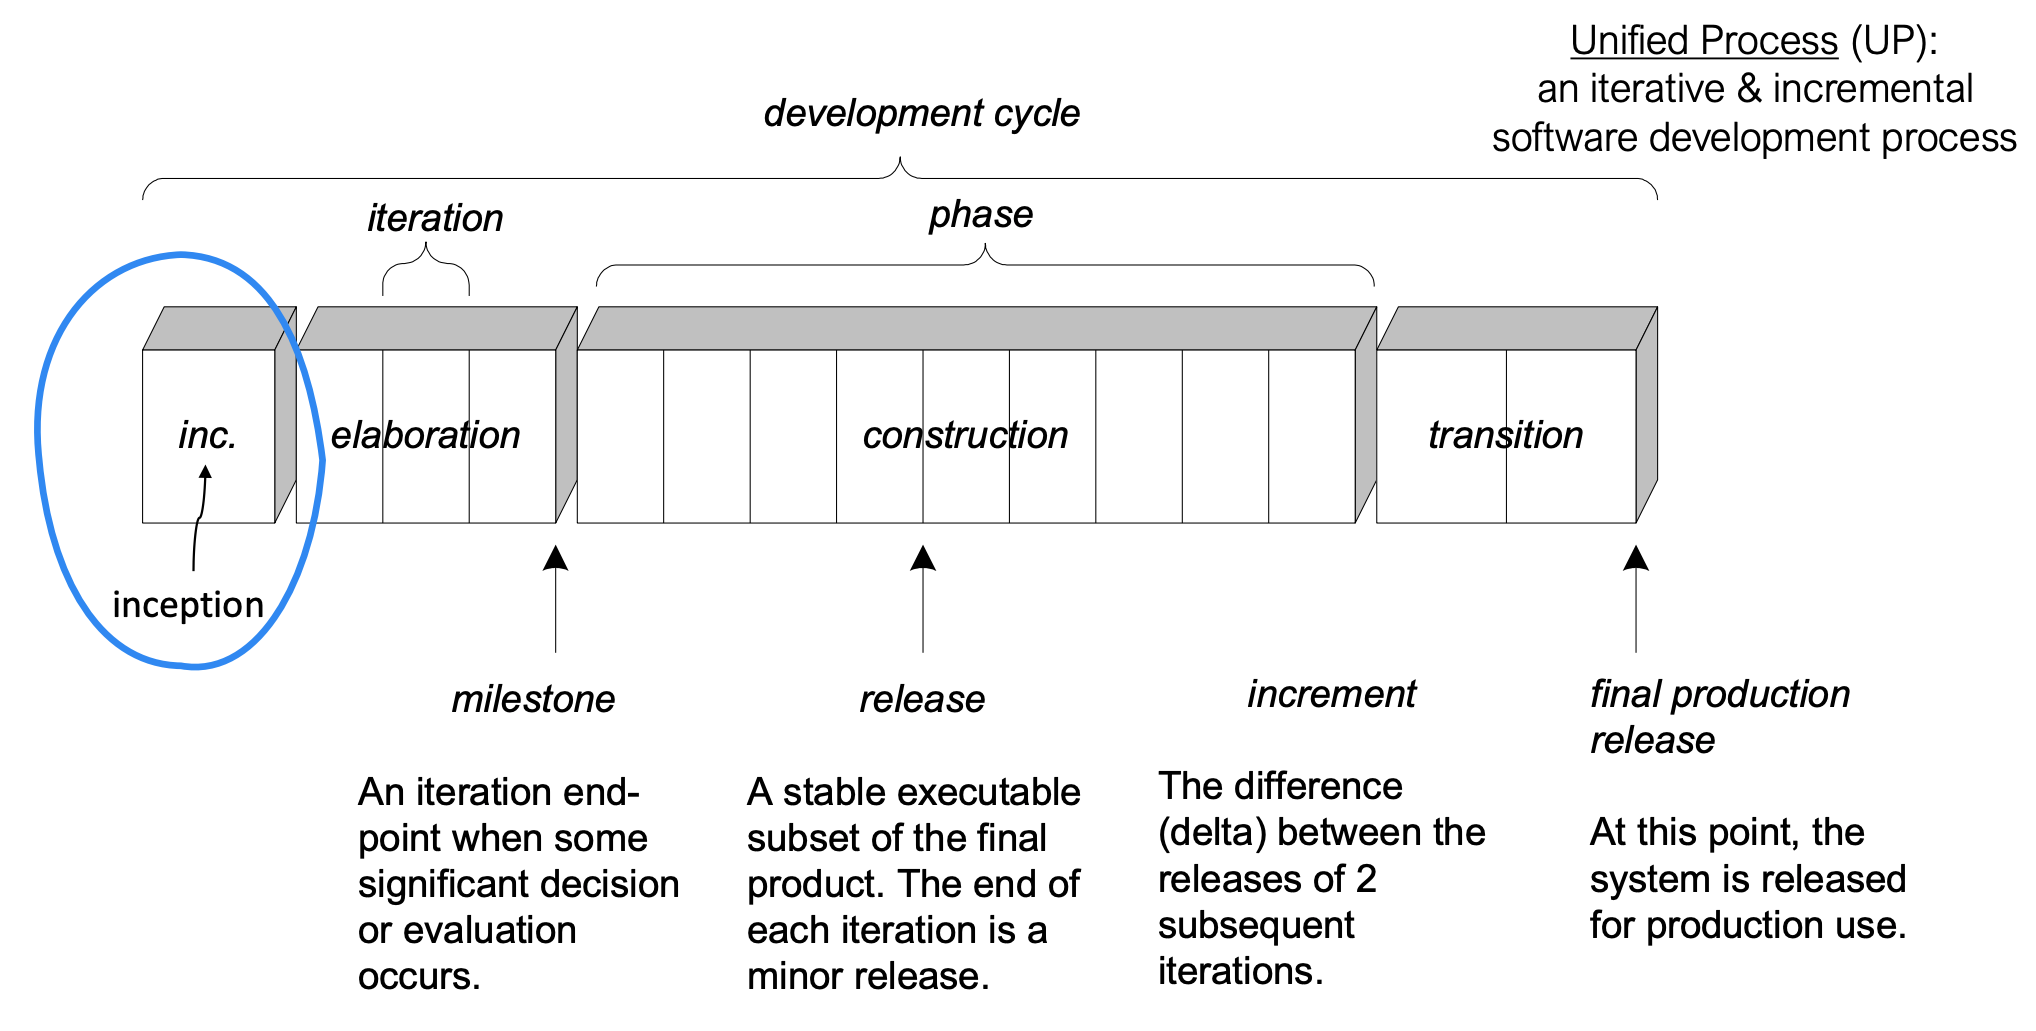
\includegraphics[width=\linewidth]{figs/unified-process.png}
\begin{enumerate}
    \item \textbf{Inception:} establish the business case for the system.
    \item \textbf{Elaboration:} develop an understanding of the problem domain and the system architecture.
    \item \textbf{Construction:} develop the system.
    \item \textbf{Transition:} deploy the system into its operating environment.
\end{enumerate}
